\section{Значение игры}

\qquad В предыдущих пунктах были найдены оптимальные стратегии для 
модельной игры с двумя различными значениями параметра дискретизации:
Т=1 и Т=2. Теперь опишем значения игры для оптимальных стратегий при
различных параметрах Т.

\subsection{Значение игры для игрока Студент}

\qquad Начнём рассмотрение со случая, когда параметр дискретизации
Т=1. На квадрате $(\mu, \lambda) \in [0, 1]^2$ мы рассмотрели
все точки и для каждой нашли оптимальные пары 
$\big(p^0(\mu, \lambda), q^0(\mu, \lambda)\big)$.
Теперь для всех возможных пар из квадрата
$(\mu, \lambda) \in [0, 1]^2$ в соответствующих
оптимальных парах найдём значения скаляризованно функции выигрыша 
игрока \textbf{С}:
$$
	\overline G(p^0(\mu, \lambda), q^0(\mu, \lambda), \mu)=
	p \min \Big\{
		\dfrac{q^0}{\mu};
		\dfrac{1-q^0}{2(1-\mu)}
	\Big\} + (1 - p^0) \min \Big\{
		\dfrac{q^0}{2\mu};
		\dfrac{1 - q^0}{1 - \mu}
	\Big\}
$$
Получим следующую систему в зависимости от значений  $\mu$ и $\lambda$:
$$
	\overline G(p^0(\mu, \lambda), q^0(\mu, \lambda), \mu) =
	\begin{cases}
		\dfrac{1}{2}, & 
		\mu = \{0,1\}, \, \lambda \in [0, 1) 
		\\	
		[\frac{1}{2}, 1], & 
		\mu = 0, \, \lambda = 1 \cup 
		\mu = 1, \, \lambda = 0
		\\
		\dfrac{1}{2-\mu}, &	
		\mu \in (0, 1), \, \lambda \in 
		(0, 2\dfrac{1 - \mu}{2 - \mu})
		\\
		\dfrac{1}{1 + \mu}, & 
		\mu \in (0, 1), \, \lambda \in 
		(\dfrac{1 - \mu}{1 + \mu}, 1]
		\\
		\Big[\dfrac{1}{2}, \, \dfrac{1}{2-\mu}\Big], &
		\mu \in (0, 1), \lambda \in 2\dfrac{1 - \mu}{2 - \mu}
		\\ 
		\Big[\dfrac{1}{2}, \, \dfrac{1}{1+\mu}\Big], &
		\mu \in (0,1), \lambda = \dfrac{1-\mu}{1+\mu}
	\end{cases}
$$

Для наглядности и дальнейшего анализа изобразим графически множество
значений выигрыша в оптимальных точках.
Для этого на квадрате $[0, 1]^{2}$ изобразим все значения, которые 
принимает вектор 
$$
	(\mu \overline G(p^0(\mu, \lambda), q^0(\mu, \lambda), \mu)), 
	(1-\mu) \overline G(p^0(\mu, \lambda), q^0(\mu, \lambda), \mu))
$$ 
при всех возможных $(\mu, \lambda) \in [0, 1]^2$. Соответствующий график
изображён на\\ рис. \ref{fig:EG_1}.

\begin{figure}[H]
	\centering
	\begin{subfigure}[b]{0.47 \textwidth}
		\centering		
		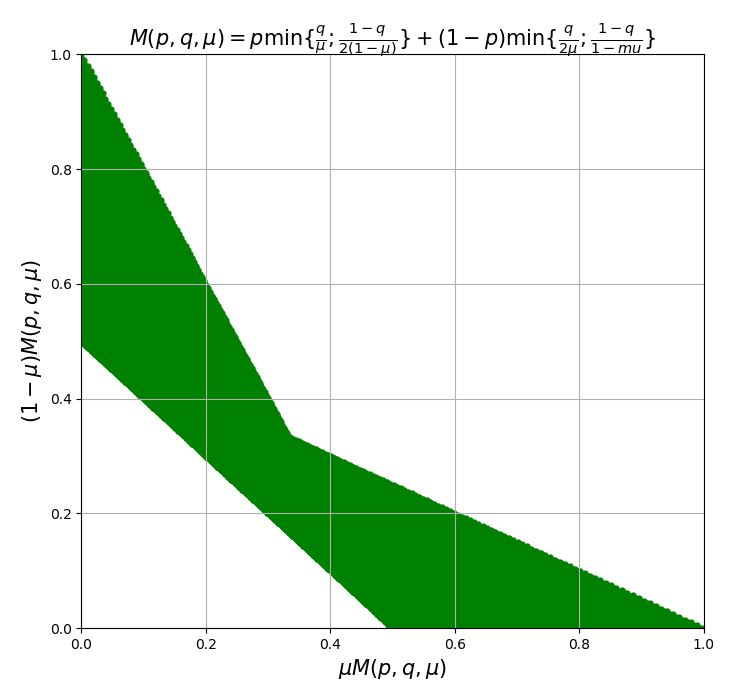
\includegraphics[width=\textwidth]{part_2/graf_4}
		\caption{}
		\label{fig:EG_1}
	\end{subfigure}	
	\begin{subfigure}[b]{0.47 \textwidth}
		\centering		
		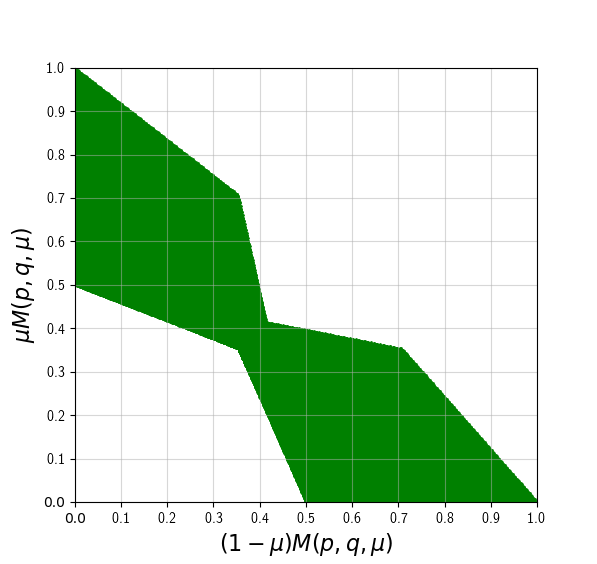
\includegraphics[width=\textwidth]{part_3/Figure_4}
		\caption{}
		\label{fig:EG_2}
	\end{subfigure}
	\caption{}	
\end{figure}

\begin{flushleft}
	Поясним график (рис. \ref{fig:EG_1}): \\
	нижняя огибающая в координатах $X,Y$: $y=\dfrac{1}{2}-x$, \\
	верхняя огибающая в координатах $X,Y$: 
	$y=
	\begin{cases}
		1 - 2x, & x \in [0, \frac{1}{3}) \\
		\dfrac{1 - x}{2}, & x \in [\frac{1}{3}, 1]
	\end{cases}
$
\end{flushleft}

Исходя из аналогичных рассуждений получим график для случая Т=2. 
Он изображён на рис. \ref{fig:EG_2}.

